\documentclass[oneside,10pt]{article}

\usepackage{url}
\usepackage{graphicx}
\usepackage[10,sharp]{easylist}
\usepackage[margin=0.7in]{geometry}   % margins
\usepackage{fancyhdr}
\usepackage[T1]{fontenc}
\usepackage{multirow}
\usepackage{hhline}
\usepackage{minted}
\usepackage{xcolor}
\usepackage{dsfont}
\usepackage{colortbl}
\pagestyle{fancy}
\usepackage{hyperref}
\usepackage{bm}
\hypersetup{
    colorlinks,
    citecolor=black,
    filecolor=black,
    linkcolor=black,
    urlcolor=black
}

\renewcommand{\baselinestretch}{1}

\definecolor{bg}{rgb}{.9,.9,.9}

\newcommand{\mf}{\mathbf}
\newcommand{\mc}{\mathcal}

\newcommand{\mi}{\mintinline{c++}}
\newcommand{\mim}{\mintinline{matlab}}
\newcommand{\mip}{\mintinline{python}}
\newcommand{\mic}{\mintinline{toml}}


\newenvironment{eq}{\begin{equation}}{\end{equation}}


% top page headers
% =============================================
\fancyhf{}
\fancyhead[EL]{\thepage}
\fancyhead[ER]{\nouppercase{\leftmark}}
\fancyhead[OL]{\nouppercase{\rightmark}}
\fancyhead[OR]{\thepage}
\renewcommand{\sectionmark}[1]{
\markboth{\thesection{} #1}{\thesection{} #1}
}
\renewcommand{\subsectionmark}[1]{
\markright{\thesubsection{} #1}
}

% top page headers
% =============================================
\RequirePackage[calcwidth]{titlesec}
\titleformat{\section}[hang]{\sffamily\bfseries}
{\Large\thesection}{12pt}{\Large}[{\titlerule[0.5pt]}]
\titleformat{\subsection}[hang]{\sffamily\bfseries}
{\large\thesubsection}{11pt}{\large}


\usepackage{cite}
\usepackage{subfigure}

\begin{document}

\title{\textbf{CLEESE} {\large v2.0} \\ {\Large A Python toolbox for random and
deterministic sound and image transformations}}
\author{February 2022}
\date{}
\maketitle

\tableofcontents

\section{Introduction}

CLEESE (Combinatorial Expressive Speech Engine) is a sound and image
manipulation tool designed to generate an infinite number of possible stimuli;
be it natural-sounding expressive variations around an original speech
recording, or variations on the expression of a human face.

More precisely, CLEESE is currently composed of two engines:
\texttt{PhaseVocoder} and \texttt{Mediapipe}.

\begin{itemize}
    \item \texttt{PhaseVocoder} allows one to create random fluctuations around
        an audio file's original contour of pitch, loudness, timbre and speed
        (i.e.\ roughly defined, its prosody). One of its foreseen applications
        is the generation of very many random voice stimuli for reverse
        correlation experiments.
    \item \texttt{Mediapipe} uses mediapipe's Face Mesh API to introduce random
        or precomputed deformation in the expression of a visage on an image.
        This engine was designed to produce batches of deformed faces for
        reverse correlation experiments.
\end{itemize}

CLEESE's \texttt{PhaseVocoder} operates by generating a set of random
breakpoint functions (BPFs) in the appropriate format for each treatment, which
are then passed to the included spectral processing engine (based on a Phase
Vocoder) with the corresponding parameters. Alternatively, the BPFs can be
externally created by the user, and so it can also be used as a Phase
Vocoder-based effects unit.

Meanwhile, CLEESE's face deformation engine works by first identifying a set of
landmarks on the visage present in the image. Then a gaussian distribution of
deformation vectors is applied to a subset of landmarks, and a Moving Least
Squares (MLS) algorithm is used to apply the deformation to the image itself.
Alternatively, a precomputed set of deformations can also be provided.

CLEESE is a free, standalone Python module, distributed under an open-source
MIT Licence on the IRCAM Forumnet plateform. It was designed by Juan José
Burred, Emmanuel Ponsot and Jean-Julien Aucouturier (STMS, IRCAM/CNRS/Sorbonne
Université, Paris), with collaboration from Pascal Belin (Institut des
Neurosciences de la Timone, Aix-Marseille Université), with generous funding
from the European Research Council (CREAM 335536, 2014--2019, PI: JJ
Aucouturier), and support for face deformation was added by Lara Kermarec
(2022). The toolbox requires Numpy, Scipy, and Mediapipe.



\section{Common configuration}\label{sec:common_conf}

In order to configure the different tools it provides, CLEESE uses
\texttt{toml} configuration files. Most sections in these file are specific to
certain engines, but here are a few variables shared among all engines:

\vspace{5pt}
\begin{minted}[bgcolor=bg]{toml}
[main]

# output root folder
outPath = "./CLEESE_output_data/"

# number of output files to generate (for random modifications)
numFiles = 10

# generate experiment folder with name based on current time
generateExpFolder = true
\end{minted}

Enabling the \texttt{generateExpFolder} option will generate a new folder
inside \texttt{outPath} for each subsequent experiment. Whereas if this option
is disabled, all experiment results are written directly in \texttt{outPath}.

\section{\texttt{PhaseVocoder} engine}
\subsection{Operation modes}

CLEESE can be used in several different modes, depending on how the main
processing function is called. Examples of several typical usage scenarios are
included in the example script \texttt{run\_cleese.py}.

\subsubsection{Batch generation}

In batch mode, CLEESE's \texttt{PhaseVocoder} engine generates many random
modifications from a single input sound file, called the base sound. It can be
launched as follows:

\vspace{8pt}
\begin{minted}[bgcolor=bg]{python}
import cleese_stim as cleese
from cleese_stim.engines import PhaseVocoder

inputFile  = 'path_to_input_sound.wav'
configFile = 'path_to_config_file.toml'

cleese.generate_stimuli(PhaseVocoder, inputFile, configFile)
\end{minted}
\vspace{8pt}


Two parameters have to be set by the user:

\vspace{5pt}
\begin{easylist}[itemize]
# \texttt{inputFile}: the path to the base sound, which has to be a mono sound in WAV format.
# \texttt{configFile}: the path to the configuration file
\end{easylist}
\vspace{8pt}

All the generation parameters for all treatments are set up in the
configuration file that has to be edited or created by the user. An example of
configuration file with parameters for all treatments is included with the
toolbox: \texttt{cleese-phase-vocoder.toml}. Configuration parameters will be
detailed in Sect. \ref{sec:pars}.

For each run in batch mode, the toolbox generates the following folder
structure, where \texttt{<outPath>} is specified in the parameter file:

\begin{sloppypar}
\vspace{5pt}
\begin{easylist}[itemize]
# \texttt{<outPath>/<currentExperimentFolder>}: main folder for the current
        generation experiment. The name \texttt{<currentExperimentFolder>} is
        automatically created from the current date and time. This folder
        contains:
## \texttt{<baseSound>.wav}: a copy of the base sound used for the current experiment
## \texttt{*.toml}: a copy of the configuration script used for the current experiment
## One subfolder for each one of the performed treatments, which can be either
        \texttt{pitch},  \texttt{eq}, \texttt{stretch} or \texttt{gain}, or a
        combination (chaining) of them. Each of them contains, for each
        generated stimulus:
### \texttt{<baseSound>.xxxxxxxx.<treatment>.wav}: the generated stimulus, where
        \texttt{xxxxxxxx} is a running number (e.g.: \texttt{cage.00000001.stretch.wav})
### \texttt{<baseSound>.xxxxxxxx.<treatment>BPF.txt}: the generated BPF, in ASCII
        format, for the generated stimulus (e.g.: \texttt{cage.00000001.stretchBPF.txt})
\end{easylist}
\vspace{8pt}
\end{sloppypar}

\subsubsection{Passing a given BPF}

When passing the \texttt{BPF} argument to \texttt{cleese.generate\_stimuli}, it
is possible to impose a given BPF with a certain treatment to an input file. In
this way, the toolbox can be used as a traditional effects unit.

\vspace{8pt}
\begin{minted}[bgcolor=bg]{python}
import numpy as np

import cleese_stim as cleese
from cleese_stim.engines import PhaseVocoder

inputFile  = 'path_to_input_sound.wav'
configFile = 'path_to_config_file.toml'

givenBPF = np.array([[0.,0.],[3.,500.]])
cleese.generate_stimuli(PhaseVocoder, inputFile, configFile, BPF=givenBPF)
\end{minted}
\vspace{8pt}

The \mip{BPF} argument can be either:
\vspace{5pt}
\begin{easylist}[itemize]
# A Numpy array containing the BPF, in the format specified in Sect.~\ref{sec:bpf}
# A scalar, in which case the treatment performed is static
\end{easylist}
\vspace{8pt}

In this usage scenario, only one file is output, stored at the
\texttt{<outPath>} folder, as specified in the configuration file.

\subsubsection{Passing a given time vector}

Instead of passing a full BPF (time+values), it is also possible to just pass a
given time vector, containing the time instants (in seconds), at which the
treatments change. The amount of modification will be randomly generated, but
they will always happen at the given time tags. This might be useful to perform
random modifications at specific onset locations, previously obtained manually
or automatically.

The time vector is passed via the \texttt{timeVec} argument:

\vspace{8pt}
\begin{minted}[bgcolor=bg]{python}
import numpy as np

import cleese_stim as cleese
from cleese_stim.engines import PhaseVocoder

inputFile  = 'path_to_input_sound.wav'
configFile = 'path_to_config_file.toml'

givenTimeVec = np.array([0.1,0.15,0.3])
cleese.generate_stimuli(PhaseVocoder, inputFile, configFile, timeVec=givenTimeVec)
\end{minted}
\vspace{8pt}

\subsubsection{Array input and output}

Instead of providing a file name for the input sound, it is possible to pass a
Numpy array containing the input waveform. In this case, the main function will
provide as output both the modified sound and the generated BPF as Numpy
arrays. No files or folder structures are created as output:

\vspace{8pt}
\begin{minted}[bgcolor=bg]{python}
import cleese_stim as cleese
from cleese_stim.engines import PhaseVocoder

inputFile  = 'path_to_input_sound.wav'
configFile = 'path_to_config_file.toml'

waveIn,sr,__ = PhaseVocoder.wavRead(inputFile)
waveOut,BPFout = cleese.process_data(PhaseVocoder,
                                     waveIn,
                                     configFile,
                                     sample_rate=sr)
\end{minted}
\vspace{8pt}

Note that the sampling rate \texttt{sample\_rate} has to be passed as well! Like
when passing a BPF, only a single sound is generated.



\subsection{Configuration file}\label{sec:pars}

All the generation parameters are set in the configuration file. Please refer
to the included configuration script \texttt{cleese-phase-vocoder.toml} for an
example.

\subsubsection{Main parameters}

The main parameters are set as follows, ignoring the parameter already
discussed in Sect.~\ref{sec:common_conf}:

\vspace{5pt}
\begin{minted}[bgcolor=bg]{toml}
[main]
# apply transformation in series (True) or parallel (False)
chain = true

# transformations to apply
transf = ["stretch", "pitch", "eq", "gain"]

[analysis]
# analysis window length in seconds
# (not to be confused with the BPF processing window lengths)
window.len = 0.04

# number of hops per analysis window
oversampling = 8
\end{minted}

\paragraph*{Chaining of transformations}~\\

If \texttt{chain} is set to \mic{true}, the transformations specified in the
\texttt{transf} list will be applied as a chain, in the order implied by the
list. For instance, the list \mic{['stretch','pitch','eq','gain']} will produce
the output folders \texttt{stretch}, \texttt{stretch\_pitch},
\texttt{stretch\_pitch\_eq} and \texttt{stretch\_pitch\_eq\_gain}, each one
containing an additional step in the process chain.

If \texttt{chain} is set to \mic{false}, the transformations will be in parallel
(all starting from the original sound file), producing the output folders
\texttt{stretch}, \texttt{pitch}, \texttt{eq} and \texttt{gain}.

\subsubsection{Common parameters}

The following parameters are shared by all treatments, but can take different values for each of them. Treatment-specific parameters will be covered in Sect. \ref{sec:treatments}.

In the following, \texttt{<treatment>} has to be replaced by one of the strings in \mic{['stretch','pitch','eq','gain']}:

\vspace{5pt}
\begin{minted}[bgcolor=bg]{python}
# common treatment parameters
[<treatment>]
# BPF window in seconds. If 0 : static transformation
window.len = 0.11

# number of BPF windows. If 0 : static transformation
window.count = 6

# 's': force winlength in seconds,'n': force number of windows (equal length)
window.unit = 'n'

# standard deviation (cents) for each BPF point of the random modification
std = 300

# truncate distribution values (factor of std)
trunc = 1

# type of breakpoint function:
#      'ramp': linear interpolation between breakpoints
#      'square': square BPF, with specified transition times at edges
BPFtype = 'ramp'

# in seconds: transition time for square BPF
trTime = 0.02
\end{minted}

\vspace{10pt}
\begin{easylist}[itemize]
# \texttt{window.len}: Length in seconds of the treatment window (i.e., the
        window used to generate the timestamps in the BPFs~-- see
        Sect.~\ref{sec:bpf}). It should be longer than
        \texttt{analysis.window.len}. This is only used if \mic{window.unit =
        's'} (see below).
## Static treatment: if \mic{window.length = 0}, the treatment is static (flat BPF).
# \texttt{window.count}: Total number of treatment windows. This is only used
        if \mic{window.unit = 'n'} (see below).
## Static treatment: if \mic{window.count = 0}, the treatment is static (flat BPF).
# \texttt{window.unit}: Whether to enforce window length in seconds (\mic{'s'})
        or integer number of windows (\mic{'n'}).
# \texttt{std}: Standard deviation of a Gaussian distribution from which the
        random values at each timestamp of the BPFs will be sampled. The unit
        of the std is specific to each treatment:
## For \texttt{pitch}: cents
## For \texttt{eq} and \texttt{gain}: amplitude dBs
## For \texttt{stretch}: stretching factor (~>1: expansion, <1: compression)
# \texttt{trunc}: Factor of the std above which distribution samples are not
        allowed. If a sample is higher than \mip{std * trunc}, a new random value
        is sampled at that point.
# \texttt{BPFtype}: Type of BPF. Can be either \texttt{ramp} or \texttt{square}
        (see Sect. \ref{sec:bpf}).
# \texttt{trTime}: For BPFs of type \texttt{square}, length in seconds of the
        transition phases.
\end{easylist}
\vspace{8pt}

\subsection{BPFs}\label{sec:bpf}

In CLEESE, sound transformations can be time-varying: the amount of
modification (e.g. the pitch shifting or time stretching factors) can
dynamically change over the duration of the input sound file. The breakpoint
functions (BPFs) determine how these modifications vary over time. For the
\texttt{pitch}, \texttt{stretch} and \texttt{gain} treatments, BPFs are
one-dimensional (temporal). For the \texttt{eq} treatment, BPFs are
two-dimensional (spectro-temporal).

As has been seen, BPFs can be either randomly generated by CLEESE or provided
by the user.

\subsubsection{Temporal BPFs}

For the \texttt{pitch}, \texttt{stretch} and \texttt{gain} treatments, BPFs are
temporal: they are two-column matrices  with rows of the form:

\begin{figure}[ht!]
\center
\subfigure[Ramp BPF with window specified in seconds]{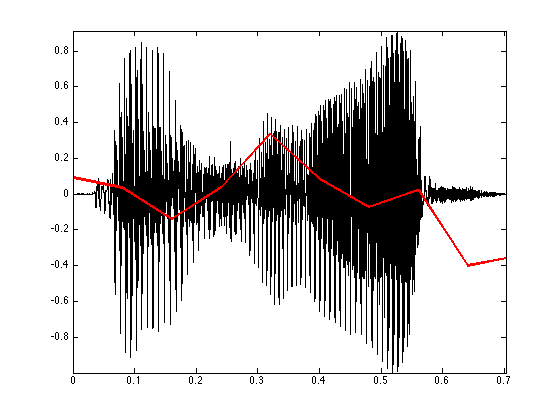
\includegraphics[height=6cm]{graph/ramps_s.png}\label{fig:ramps_s}}
\subfigure[Ramp BPF with window specified in number]{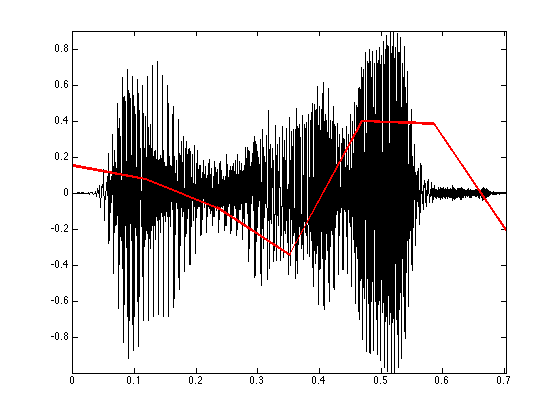
\includegraphics[height=6cm]{graph/ramps_n.png}\label{fig:ramps_n}}
\subfigure[Square BPF with window specified in seconds]{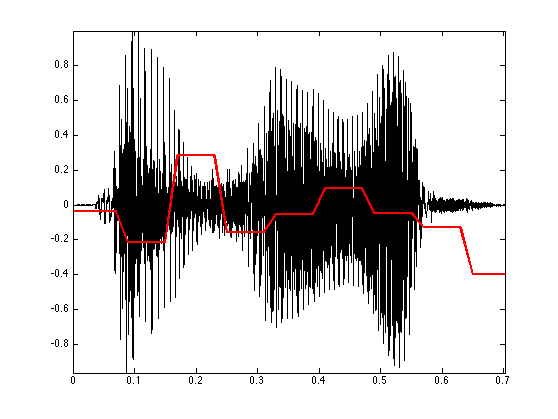
\includegraphics[height=6cm]{graph/square_s}\label{fig:square_s}}
\subfigure[Square BPF with window specified in number]{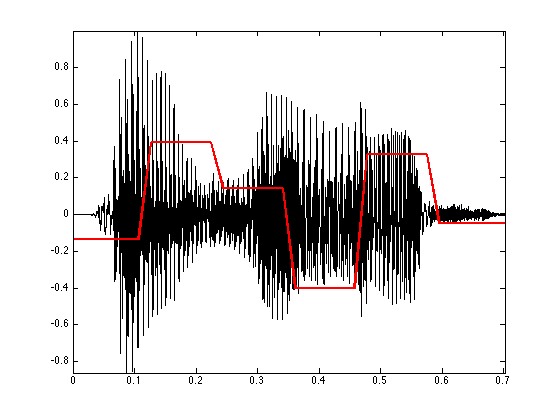
\includegraphics[height=6cm]{graph/square_n}\label{fig:square_n}}
\caption{Examples of randomly generated temporal BPFs.}\label{fig:bpf}
\end{figure}


\vspace{8pt}
 \mip{time value}
\vspace{8pt}

\texttt{time} is in seconds, and \texttt{value} is in the same units than the
\texttt{std} parameter. CLEESE can randomly generate one-dimensional BPFs of
two types:

\vspace{5pt}
\begin{easylist}[itemize]
# \textbf{Ramps} (\mic{BPFtype = 'ramp'}): the BPF is interpreted as a linearly
        interpolated function. The result is that the corresponding sound
        parameter is changed gradually (linearly) between timestamps. Examples
        are shown on Fig.~\ref{fig:ramps_s} for a treatment window defined in
        terms of seconds (\mic{window.unit = 's'}), and on
        Fig.~\ref{fig:ramps_n} for a treatment window defined in terms of
        window number (\mic{window.unit = 'n'}). Note that in the first case,
        the length of the last window depends on the length of the input sound.
        In the second case, all windows have the same length.
# \textbf{Square} (\mic{BPFtype = 'square'}): the BPF is a square wave with
        sloped transitions, whose length is controlled by \texttt{trTime}.
        Examples are shown on Fig.~\ref{fig:square_s} for a treatment window
        defined in terms of seconds (\mic{window.unit = 's'}), and on
        Fig.~\ref{fig:square_n} for a treatment window defined in terms of
        window number (\mic{window.unit = 'n'}).
\end{easylist}
\vspace{8pt}

\subsubsection{Spectro-temporal BPFs}\label{sec:bpf_2d}

The \texttt{eq} treatment performs time-varying filtering over a number of
determined frequency bands. It thus expects a spectro-temporal
(two-dimensional) BPF whose rows are defined as follows:

\vspace{8pt}
\texttt{time numberOfBands freq1 value1 freq2 value2 freq3 value3 ...}
\vspace{8pt}

The temporal basis can again be generated as \texttt{ramp} or \texttt{square}.
In contrast, in the frequency axis, points are always interpolated linearly.
Thus, a spectro-temporal BPF can be interpreted as a time-varying
piecewise-linear spectral envelope.

\subsection{Treatments}\label{sec:treatments}

\subsubsection{Time stretching (\texttt{stretch})}

This treatment stretches or compresses locally the sound file without changing
the pitch, according to the current stretching factor (oscillating around 1) at
the current timestamp. This is the only treatment that changes the duration of
the output compared to the base sound. The used algorithm is a phase vocoder
with phase locking based on frame-wise peak picking.

\subsubsection{Pitch shifting (\texttt{pitch})}

The BPF is used to transpose up and down the pitch of the sound, without
changing its duration. The used algorithm is a phase vocoder with phase locking
based on frame-wise peak picking, followed by resampling on a window-by-window
basis.

\subsubsection{Time-varying equalization (\texttt{eq})}

This treatment divides the spectrum into a set of frequency bands, and applies
random amplitudes to the bands. The definition of band edges is constant, the
amplitudes can be time-varying. The corresponding BPF is thus two-dimensional
and follows the format described in Sect.~\ref{sec:bpf_2d}.

There are two possible ways to define the band division:

\vspace{5pt}
\begin{easylist}[itemize]
# \textbf{Linear} division into a given number of bands between 0 Hz and Nyquist.
# Division according to a \textbf{mel} scale into a given number of bands. Note
        that it it possible to specify any number of filters (less or more than
        the traditional 40 filters for mel cepstra).
\end{easylist}
\vspace{8pt}

These settings are defined by the following treatment-specific parameters:

\vspace{5pt}
\begin{minted}[bgcolor=bg]{toml}
[eq]
scale = 'mel'  # mel, linear
band.count = 10
\end{minted}

\subsubsection{Time-varying gain (\texttt{gain})}

For gain or level randomization, the BPF is interpolated and interpreted as an
amplitude modulator. Note that the corresponding standard deviation is
specified in dBs (base-10 logarithm). If the resulting output exceeds the
maximum float amplitude of \mic{1.0}, the whole output signal is normalized.


\section{\texttt{Mediapipe} engine}
\subsection{Operation modes}

CLEESE can be used in different modes, depending on which function you call and
how. Examples of several typical usage scenarios are include in the example
script \texttt{run\_cleese.py}.

\subsubsection{Batch generation}

CLEESE has a dedicated function for batch treatments:
\texttt{cleese.generate\_stimuli}, which is used, in \texttt{Mediapipe}'s case,
to generate a number of randomly deformed visages.

\vspace{8pt}
\begin{minted}[bgcolor=bg]{python}
import cleese_stim as cleese
from cleese_stim.engines import Mediapipe

inputFile  = 'path_to_input_image.jpg'
configFile = 'path_to_config_file.toml'

cleese.generate_stimuli(Mediapipe, inputFile, configFile)
\end{minted}
\vspace{8pt}

Two parameters have to be set by the user:

\vspace{5pt}
\begin{easylist}[itemize]
# \texttt{inputFile}: the path to the base image, which can be any image format
        readable and writeable by \texttt{PIL}.
# \texttt{configFile}: the path to the configuration script
\end{easylist}
\vspace{8pt}

All the generation parameters for all treatments are set up in the
configuration script that has to be edited or created by the user. An example
of configuration script with parameters for all treatments is included with the
toolbox: \texttt{cleese-mediapipe.toml}. Configuration parameters will be
detailed in Sect.~\ref{sec:mediapipe:conf}.

For each run in batch mode, the toolbox generates the following folder
structure, where \texttt{<outPath>} is specified in the parameter file:

\begin{sloppypar}
\vspace{5pt}
\begin{easylist}[itemize]
# \texttt{<outPath>/<currentExperimentFolder>}: main folder for the current
        generation experiment. The name \texttt{<currentExperimentFolder>} is
        automatically created from the current date and time. This folder
        contains:
## \texttt{<baseImage.ext>}: a copy of the base image used for the current experiment
## \texttt{*.toml}: a copy of the configuration script used for the current experiment
## \texttt{<baseimage>.xxxxxxxx.<ext>}: the generated deformed image, where
        \texttt{xxxxxxxx} is a running number (e.g.:
        \texttt{monalisa.00000001.jpg})
## \texttt{<baseimage>.xxxxxxxx.dfmxy}: the generated deformation vectors, in
        CSV format, for the generated stimulus (e.g.:
        \texttt{monalisa.00000001.dfmxy})
## \texttt{<baseimage>.landmarks.txt}: the list of all landmarks positions as
        detected on the original image, in ASCII format, readable with
        \texttt{numpy.loadtxt}.
\end{easylist}
\vspace{8pt}
\end{sloppypar}

\subsubsection{Array input and output}

CLEESE can also provide a single result, based on data loaded previously in a
script or directly loading a file.

\paragraph*{From array}~\\

Here, you can also use \texttt{PIL.Image}'s
\mip{np.array(Image.open("path/image.jpg").convert("RGB"))} to load the image.
The Face Mesh API requires that the image be in RGB format.

\vspace{8pt}
\begin{minted}[bgcolor=bg]{python}
import cleese_stim as cleese
from cleese_stim.engines import Mediapipe

inputFile  = 'path_to_input_image.jpg'
configFile = 'path_to_config_file.toml'

img = Mediapipe.load_file(inputFile)
deformedImg = cleese.process_data(Mediapipe, img, configFile)
\end{minted}
\vspace{8pt}

\paragraph*{From file}~\\

\vspace{8pt}
\begin{minted}[bgcolor=bg]{python}
import cleese_stim as cleese
from cleese_stim.engines import Mediapipe

inputFile  = 'path_to_input_image.jpg'
configFile = 'path_to_config_file.toml'

deformedImg = cleese.process_file(Mediapipe, inputFile, configFile)
\end{minted}
\vspace{8pt}

In both of those cases, no files or folder structures are generated.

\subsubsection{Applying a deformation}

Both \texttt{cleese.process\_data} and \texttt{cleese.process\_file} function
allow for applying a precomputed set of deformations instead of generating them
randomly. CLEESE can accept both \texttt{.dfmxy} deformations (absolute
cartesian deformation vectors), and \texttt{.dfm} deformations (deformation
vectors mapped onto a triangulation of face landmarks (dlib landmarks
indices)).

\vspace{8pt}
\begin{minted}[bgcolor=bg]{python}
import cleese_stim as cleese
from cleese_stim.engines import Mediapipe

dfmxyFile = 'path_to_dfmxy.dfmxy'
dfmFile = 'path_to_dfm.dfm'
imageFile  = 'path_to_input_image.jpg'
configFile = 'path_to_config_file.toml'

# .dfmxy processing
dfmxy = Mediapipe.load_dfmxy(dfmxyFile)
img = cleese.process_file(Mediapipe,
                          imageFile,
                          configFile,
                          dfmxy=dfmxy)

# .dfm processing
dfm = Mediapipe.load_dfm(dfmFile)
img = cleese.process_file(Mediapipe,
                          imageFile,
                          configFile,
                          dfm=dfm)
\end{minted}
\vspace{8pt}

\subsubsection{Converting deformation files}

Other face deformation tools developed by our team use the \texttt{.dfm}
deformation file format, more suited to applying the same deformation to an
arbitrary face. However, by its use of barycentric coordinates in a landmarks
triangulation, it isn't suited to any post or pre-processing, which is an area
where \texttt{.dfmxy} shines. As a result, CLEESE's Mediapipe provides a way to
convert a given, \texttt{.dfmxy} to \texttt{.dfm}, provided you also have the
original landmarks on hand:

\vspace{8pt}
\begin{minted}[bgcolor=bg]{python}
import cleese_stim as cleese
from cleese_stim.engines import Mediapipe

dfmxyFile = 'path_to_dfmxy.dfmxy'
dfmFile = 'path_to_dfm.dfm'
landmarksFile = 'path_to_landmarks.txt'

img = cleese.dfmxy_to_dfm(dfmxyFile,
                          landmarksFile,
                          output_dfm_file=dfmFile)
\end{minted}
\vspace{8pt}

\subsection{Configuration}\label{sec:mediapipe:conf}

The following parameters are used to configure the \texttt{Mediapipe} engine:

\vspace{8pt}
\begin{minted}[bgcolor=bg]{toml}
[mediapipe.random_gen]
# Indices of the landmarks to be modified, using Dlib's 68 landmarks indexing
landmarks.dlib = []

# Indices of the landmarks to be modified, using Mediapipe's 468 landmarks indexing
landmarks.mediapipe = [61, 40, 78, 91, 270, 308, 321, 291]  # lips corners

# Sets of landmarks to be modified, using precomputed sets
# "dlib-eyebrow-right", "dlib-eyebrow-left", "dlib-nose",
# "dlib-eye-right", "dlib-eye-left", "dlib-outer-lips",
# "dlib-inner-lips", "dlib-lips", etc...
# See cleese/engines/mediapipe.py for a full list
landmarks.presets = ["dlib-lips"]

# Covariance matrix used to generate the gaussian distribution of landmarks
# offsets. It is scaled according to the height of the detected face. As a
# result, the amount of deformation should be resolution-invariant.
covMat = [[0.0002, 0.0], [0.0, 0.0002]]

[mediapipe.mls]
# Alpha parameter of the MLS deformation.
# Affects how much the deformation "spreads" from the landmarks
alpha = 1.2

[mediapipe.face_detect]
# Minimum face detection confidence
threshold = 0.5
\end{minted}
\vspace{8pt}

\vspace{10pt}
\begin{easylist}[itemize]
# \texttt{mediapipe.random\_gen.landmarks}: Selection of landmarks on which to
        apply a deformation. Then can be defined in a few different ways:
## \texttt{landmarks.dlib}: Array of landmark indices, using dlib's Multi-PIE
        68 landmarks indexing (see fig.~\ref{fig:landmarks:dlib}).
## \texttt{landmarks.mediapipe}: Array of landmark indices, using mediapipe's 468
        vertices face mesh (see google's
        \href{https://github.com/google/mediapipe/blob/master/mediapipe/modules/face_geometry/data/canonical_face_model_uv_visualization.png}{canonical\_face\_model\_uv\_visualization.jpg})
## \texttt{landmarks.presets}: Array of name of landmarks presets. For now,
        only subset of dlib's indices are implemented.
# \texttt{covMat}: The covariance matrix used when drawing the distribution of
        deformation vectors. the unit vector is scaled according to height of
        the detected face, to enable for scale-invariant deformations.
# \texttt{mediapipe.mls.alpha}: Moving Least Squares (MLS) algorithm
        alpha parameter, affecting the "spread" of the deformation.
# \texttt{mediapipe.face\_detect.threshold}: Threshold for the confidence
        metric of mediapipe's face detector. Ajust if faces aren't detected, or
        if things that aren't faces are detected.
\end{easylist}
\vspace{8pt}

\begin{figure}[ht!]
\center
\subfigure{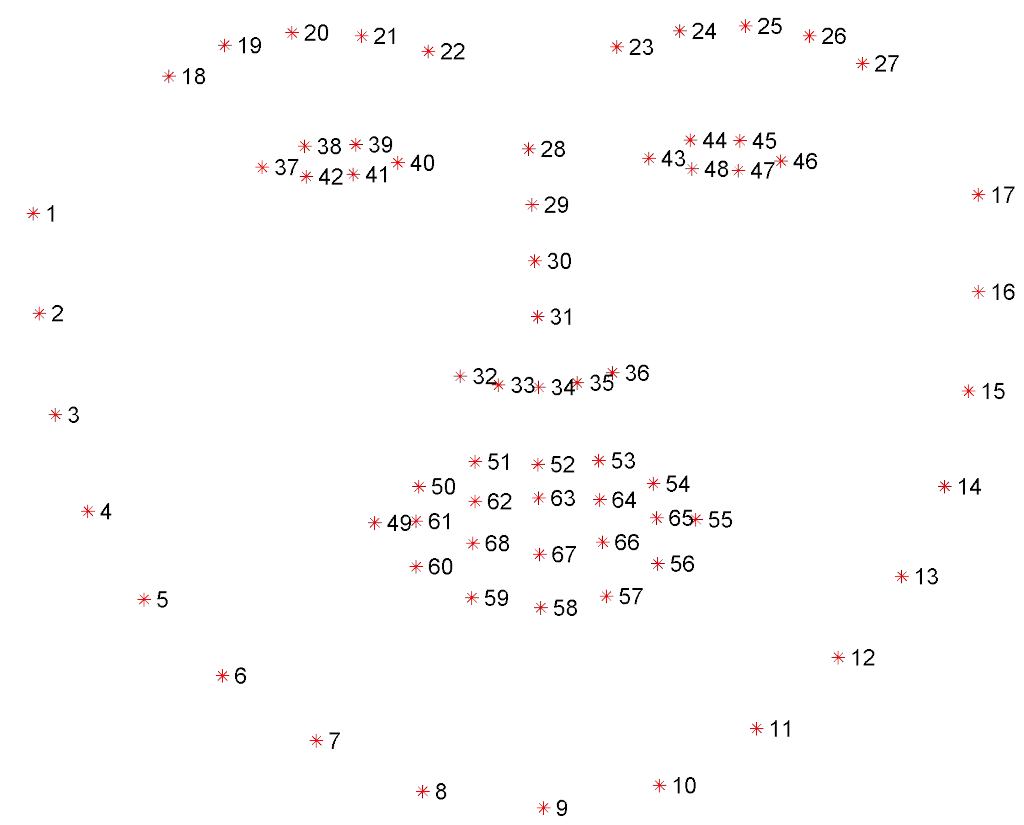
\includegraphics[height=6cm]{graph/dlib_68_landmarks.png}\label{fig:landmarks:dlib}}
\caption{Dlib's 68 Multi-PIE landmarks, 1-indexed.}
\label{fig:voronoi}
\end{figure}

\bibliography{}
\bibliographystyle{plain}

\end{document}
